%Dokumentinnstillinger:---------------------------------
%Ved å google flitting kan du finne ut hva de forskjellige tingene her betyr, og hvordan du kan gjøre eventuelle endringer.
\documentclass[a4paper,11pt,norsk]{article}
\usepackage[utf8]{inputenc}
\usepackage{a4wide}
\usepackage{lmodern}
\usepackage[T1]{fontenc}
\usepackage{babel}
\setlength{\parindent}{0pt} 
\setlength{\parskip}{2ex}
\usepackage{fixltx2e}
\usepackage{amsmath}
\usepackage[pdftex, pdfborderstyle={/S/U/W 0}]{hyperref}
\usepackage{graphicx}
\usepackage[font=small,labelfont=bf]{caption}
\usepackage{tabularx}
\usepackage{multirow}
\usepackage{float}
\usepackage{subcaption}
\usepackage[RPvoltages]{circuitikz}




\begin{document}

%Headingdel:---------------------------------------------
\begin{minipage}[c]{0.15\textwidth}

\includegraphics[width=2.0cm]{D1/Images/elsys_pos_staaende_ntnu.png}  
\end{minipage}
\begin{minipage}[c]{0.85\textwidth}

\renewcommand{\arraystretch}{1.7}
\large 
\begin{tabularx}{\textwidth}{|X|X|}
\hline
\multicolumn{2}{|l|}{} \\
\multicolumn{2}{|l|}{\huge \textbf{Designnotat}} \\
\multicolumn{2}{|l|}{}  \\
\hline
\multicolumn{2}{|l|}{Tittel: 
%Skriv inn tittel her:------------------------------------------
Impulsrespons
} \\
\hline
\multicolumn{2}{|l|}{Forfatter: 
%Skriv inn forfattere her:--------------------------------------
Freider Engstrøm Fløan
} \\
\hline
%Skriv inn versjon og dato her her:-----------------------------
Versjon: 1.0 & Dato: 16.05.22
\\
\hline 
\end{tabularx}
\end{minipage}
\normalsize

%Automatisk generert innholdsfortegnelse:------------------

\setlength{\parskip}{0ex}
\renewcommand{\baselinestretch}{0.1}\normalsize
\tableofcontents
\renewcommand{\baselinestretch}{1.00}\normalsize
\setlength{\parskip}{2ex}
\rule{\textwidth}{1pt}
\label{sec:innledning}

\newpage



%Selve rapporten:------------------------------------------
\section{Innledning}
\label{sec:problembeskrivelse}

En dirac-puls $\delta(t)$ er et matematisk objekt som aldri kan realiseres fysisk. Det er en uendelig
kort puls med uendelig stor verdi men som inneholder en endelig mengde eneregi.
Selv om dirac-pulsen ikke kan realiseres i praksis, har den en viktig teoretisk betydning. Dersom vi
tenker oss at den utgjør inngangen til et lineært tidsinvariant system\footnote{Et system som beskrives av en lineær differensialligning med konstante koeffisienter.
}
, vil utgangen av systemet
$h(t)$, som vi kaller systemets impulsrespons inneholde all informasjon om systemets egenskaper.\footnote{Dette behandles ytterligere i emne TTT4265 Elektroisk systemdesign og -analyse II.}
Se figur \ref{fig:1}.

\begin{figure}[H]
  \centering
  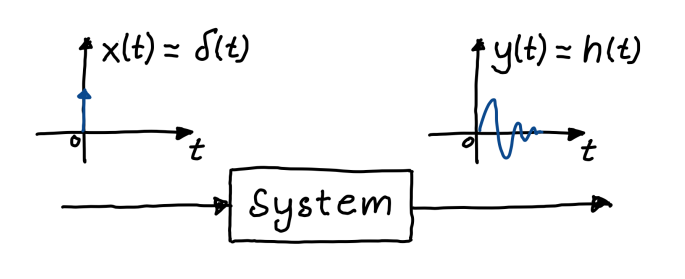
\includegraphics[scale=0.7]{D1/Images/figur 1.png}
  \caption{Når inngangen til et system har form av en dirac-puls $\delta(t)$, er utgangen per definisjon
systemets impulsrespons $h(t)$.}
  \label{fig:1}
\end{figure}

Figur \ref{fig:1}: Når inngangen til et system har form av en dirac-puls $δ(t)$, er utgangen per definisjon
systemets impulsrespons $h(t)$.
En tilnærming til impulsresponsen kan man få ved å bruke som inngangssignal en puls av endelig,
men veldig kort varighet og så registrere systemets respons. Et eksempel på en slik undersøkelse
finner vi i rom-akustikken. Da man skulle vurdere plasseringen av Wagner-orgelet i Nidaros domkirke, ble det avfyrt pistol-skudd ulike steder i bygningen for å estimere rommets impulsrespons.
For et elektronisk system kan impulresponsen undersøkes ved hjelp av en impuls-generator og et
oscilloskop som vist i figur \ref{fig:2}.

\begin{figure}[H]
  \centering
  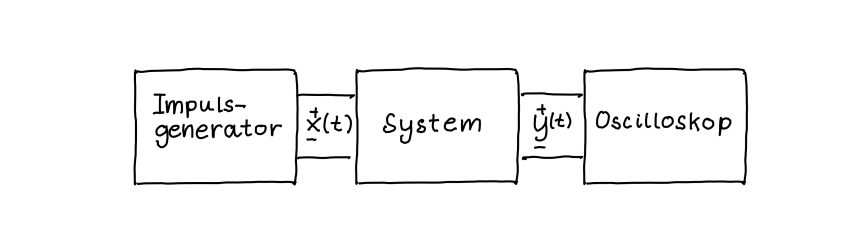
\includegraphics[scale=0.7]{D1/Images/figur 2.png}
  \caption{Undersøkelse av impulsrespons ved hjelp av impulsgenerator og oscilloskop.}
  \label{fig:2}
\end{figure}

Impulsgeneratoren produserer et signal $x(t)$ bestående av en serie korte pulser med avstand $T$. I
det teoretisk ideelle tilfellet, består $x(t)$ av uendelig korte dirac-pulser som vist i figur \ref{fig:3}. Utgangen
$y(t)$ av systemet avleses på oscilloskopet.

\begin{figure}[H]
  \centering
  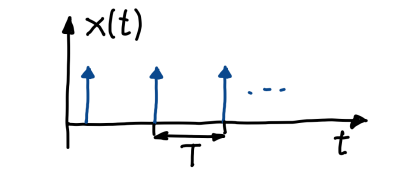
\includegraphics[scale=0.7]{D1/Images/figur 3.png}
  \caption{Sekvens av ideelle dirac-pulser
}
  \label{fig:3}
\end{figure}

En praktisk impulsgenerator vil generere korte pulser, jo kortere jo bedre. En design-ide for
en slik impulsgenerator skal undersøkes.

\section{Undersøkelser}
\label{sec:undersøkelser}
\subsubsection{Firkantgenerator} % FIRKANT
\label{firkantgenerator}

En firkantgenerator er et oscillerende system som gir ut et firkantsignal. Firkantgeneratoren som brukes, se figur \ref{fig:firkantgenerator1}, er hentet fra~\cite{Ert-18}, der perioden $T$ er gitt ved likningen:
\begin{equation}
    \text{T} = 2\text{ln}(3)\tau.
    \label{eq:T_firkant}
\end{equation}

En mulig måte å realisere en slik generator med to NOG-porter i CD4011UBE er vist i figur \ref{fig:firkantgenerator2}. 
\begin{figure}[H]
\centering
    \begin{subfigure}{0.5\linewidth}
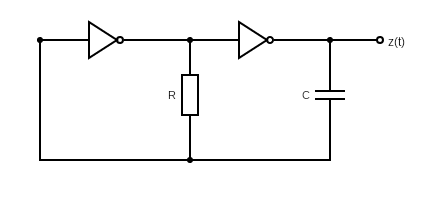
\includegraphics[width=\linewidth]{D1/Images/firkantgenerator1.png} 
    \caption{IKKE-porter.}
\label{fig:firkantgenerator1}
    \end{subfigure}\hfill
    \begin{subfigure}{0.5\linewidth}
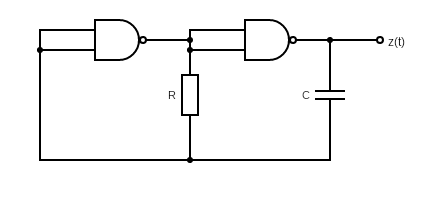
\includegraphics[width=\linewidth]{D1/Images/firkantgenerator2.png}
    \caption{NOG-porter.}
\label{fig:firkantgenerator2}
    \end{subfigure}
\caption{Kretsskjema av firkantsgenratorer med forskjellige logiske porter.}
    \label{fig:firkantgenerator}
\end{figure}

Fra~\cite{oving6} er amplitudespekteret til et firkant signal definert som:
\begin{equation}
\label{eq:c_k}
    c_k=aV_0sinc(ak),\;\;\;\;\;k=\pm1,2,3,4...
\end{equation}
når firkantsignalet er definert som:
\[ x(t) =
  \begin{cases}
    V_0       & \quad \text{for } \abs(t) < \frac{aT}{2}\\
    0  & \quad \text{for } \frac{aT}{2}< \abs(t) < \frac{T}{2}.
  \end{cases}
\]
Hvis $a \xrightarrow[]{} 0$ vil likning (\ref{eq:c_k}) gi et flatt amplitudespekter som vist i figur \ref{fig:ideeltamplitudespekter}.
\begin{figure}[H]
  \centering
  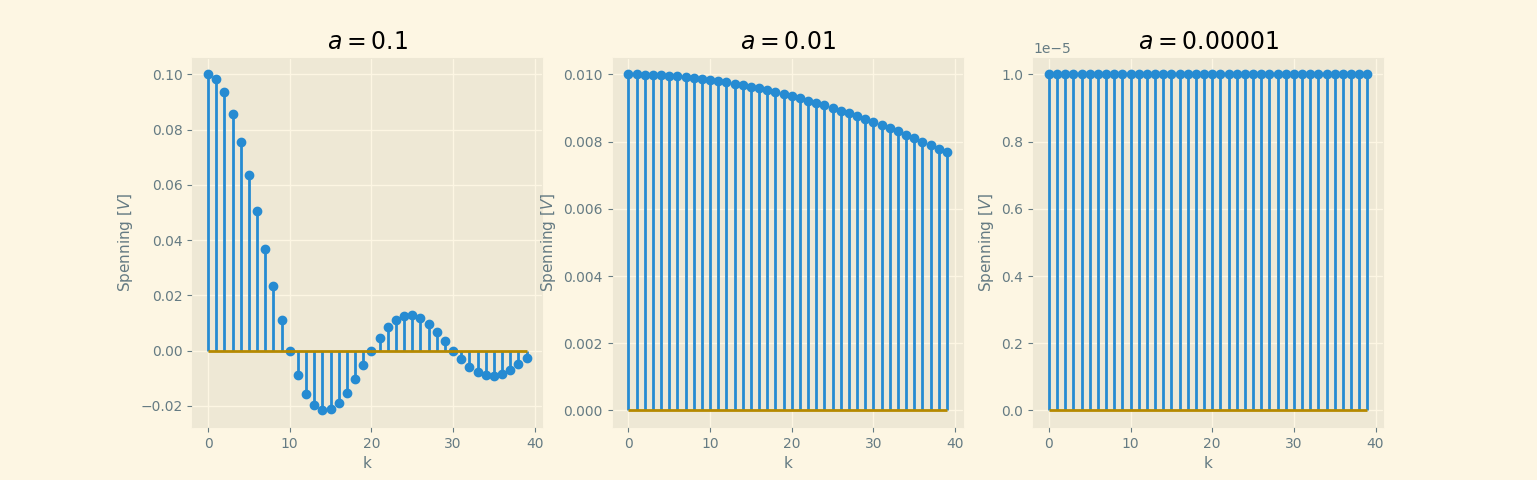
\includegraphics[scale=0.4]{D1/Images/amplitudespekter.png}
  \caption{Ampllitudespekteret til et firkantsignal der pulsbreddevariabelen $a \xrightarrow[]{} 0$.}
  \label{fig:ideeltamplitudespekter}
\end{figure}

\subsubsection{Impulsgenerator}
\label{sec:impulsgenerator}

Impulsgeneratoren som undersøkes fra~\cite{Eksamensprosjekt} er vist i figur \ref{fig:impulsegenerator1}, der inngangsignalet er fra firkantgeneratoren $z(t)$ med et RC-høypassfilter og en OG-port. Ved bruk av en  CD4011UBE, kan en tilsvarende generator designes med to NOG-porter vist i figur \ref{fig:impulsegenerator2}.

\begin{figure}[H]
\centering
    \begin{subfigure}{0.45\linewidth}
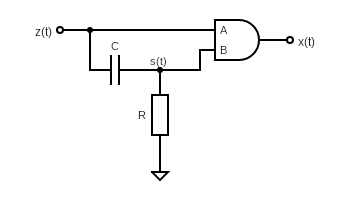
\includegraphics[width=\linewidth]{D1/Images/impulsegenerator_and.png} 
    \caption{OG-port.}
\label{fig:impulsegenerator1}
    \end{subfigure}\hfill
    \begin{subfigure}{0.55\linewidth}
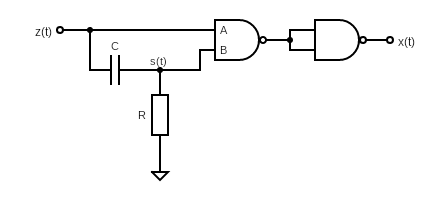
\includegraphics[width=\linewidth]{D1/Images/impulsegenerator_nand.png}
    \caption{NOG-porter.}
\label{fig:impulsegenerator2}
    \end{subfigure}
\caption{Kretsskjema av impulsegenerator med forskjellige logiske porter.}
    \label{fig:impulsgenerator}
\end{figure}

Figur \ref{fig:zsx} viser hvordan signalet fra firkantgeneratoren, $z(t)$, holder inngang A til OG-porten i figur \ref{fig:firkantgenerator} høy når $z(t)$ er høy. Inngang B på OG-porten vil være høy så lenge høypassfilteret, $s(t)$, er høyt. Høyt i dette tilfelle blir terskelspenningen til NOG-portene i CD4011UBE. Fra databladet~\cite{datablad} er terskelspenningen $V_{th}$ gitt ved $\frac{V_{DD}}{2}$ som gir at $x(t)$ er høy så lenge $s(t)$ > $\frac{V_{DD}}{2}$.

\begin{figure}[H]
    \centering
    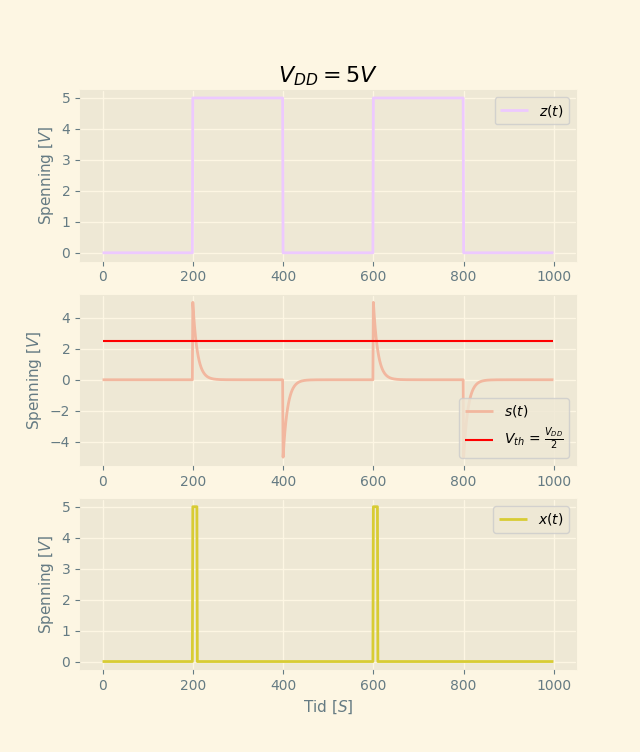
\includegraphics[scale=0.75]{D1/Images/zsx.png}
    \caption{Ideele signaler til impulsgeneratoren.}
    \label{fig:zsx}
\end{figure}

Hvis perioden $\frac{T}{2}$ til $z(t)$ blir kortere enn tiden $s(t)$ bruker på å gå under terskelspenningen vil $x(t)$ = $z(t)$. Da det er ønskelig at hver puls i $x(t)$ er så smal som mulig, må en kondensator og/eller motstand velges som har tilstrekkelig lav verdi.

For at $z(t) \neq x(t)$ må $v_C(t) < \frac{V_{DD}}{2}$ etter $\frac{T}{2}$ til firkantgeneratoren. 


Fra~\cite{Ert-19} er spenningen til en kondensator med hensyn på tid:
\begin{equation}
\label{eq:tau}
    v_c=v_c(\infty)+[v_c(0)-v_c(\infty)]e^{-\frac{t}{\tau}},\;\;\;\;\;  \tau=RC. 
\end{equation}
Ved å se på når likning (\ref{eq:tau}) er mindre enn $\frac{V_{DD}}{2}$, altså terskelspenningen til portene, kan likningen løses for $\tau$:
\begin{equation}
    \text{Når}\;\; \frac{V_{DD}}{2} > V_{DD}+[0-V_{DD}]e^{-\frac{t}{\tau}} \xrightarrow[]{}x(t)=0
\end{equation}
deler på $V_{DD}$ og får:
\begin{equation}
    \frac{1}{2} > 1-e^{-\frac{t}{\tau}}
\end{equation}
\begin{equation}
    \text{ln}(\frac{1}{2}) < -\frac{t}{\tau}
\end{equation}
\begin{equation}
    \label{eq:finishedTau}
    \text{ln}(2)\tau < t 
\end{equation}
gitt at firkantsignalet $z(t)$ går fra $0$V til $5$V der $V_{DD} = 5V$. Fra likning (\ref{eq:finishedTau}) vil korteimpulser genereres når $\tau$ er lav, som kan oppnås ved å ha lave komponentverdier på $R_2$ og $C_2$.

Grunnen til at $z(t)$ ikke går inn på begge inngangene til OG-porten er fordi det ville gitt impulser med negativ amplitude mellom hver positive impuls. 

\subsubsection{RLC-båndpassfilter}
\label{RCL-båndpassfilter}

En metode for å se hvordan et tidsinvariant system oppfører seg for alle signaler er ved å se på impulsresponsen til systemet. Systemet som skal undersøkes i denne rapporten er et RLC-båndpassfilter. Hvordan filteret fungerer er nærmere beskrevet i tidligere designnotat~\cite{D2},~\cite{D3} og~\cite{D4}. En analogi til hvordan et slik filter vil reagere på en impuls er med et legemet som henger i et tau. Hvis man da påfører en impulskraft på legeme vil det begynne å svinge, som da er kondensatoren og spolen som gir energi frem og tilbake. Hvis det ikke er luftmotstand vil legemet svinge for alltid, som tilsvarer ideele ledere uten motstand. kobler man på en motstand vil denne svingningen begynne å bremse. Motstanden tapper systemet for energi, mens kondensatoren og spolen lagrer og gir energi.

Q-verdien til et filter, gitt ved likningen:
\begin{equation}
    Q = \frac{1}{R}\sqrt{\frac{L}{C}}
\end{equation}
viser at når $R$ øker vil Q-verdien minke. Dermed vil en lav Q-verdi indikere en høy motstandsverdi som bremser eller tapper filteret for energi raskere. 

Hvis perioden $T$ til firkantsignalet $z(t)$ blir så kort at dempningene i impulsresponsen ikke rekker å bli dempet før det kommer en ny impuls vil signalene begynne å overlappe. Derfor er det viktig at firkantgeneratoren har lang nok periodetid som kan løses ved å øke $\tau$ i likning (\ref{eq:T_firkant}).

\subsection{Realisering}
\label{realisering}

For å gjennomføre de forskjellige oppgavene vil verdiene på komponentene endres, men figur \ref{fig:kretsskjema_utenverdier} viser hvordan komponentene er satt sammen med den integrerte kretsen CD4011UBE. Figur \ref{fig:oppkobling} viser realisert krets på et brødbrett med verdier brukt i tabell \ref{tab:komp} under.  
\begin{figure}
    \centering
    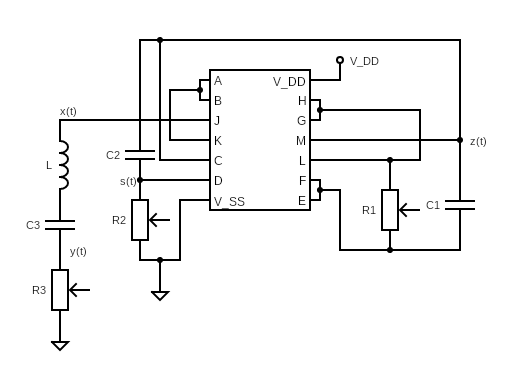
\includegraphics[scale=0.7]{D1/Images/circuitWithoutValues.png}
    \caption{Kretsskjema av fullstendig krets.}
    \label{fig:kretsskjema_utenverdier}
\end{figure}

\begin{figure}[H]
  \centering
  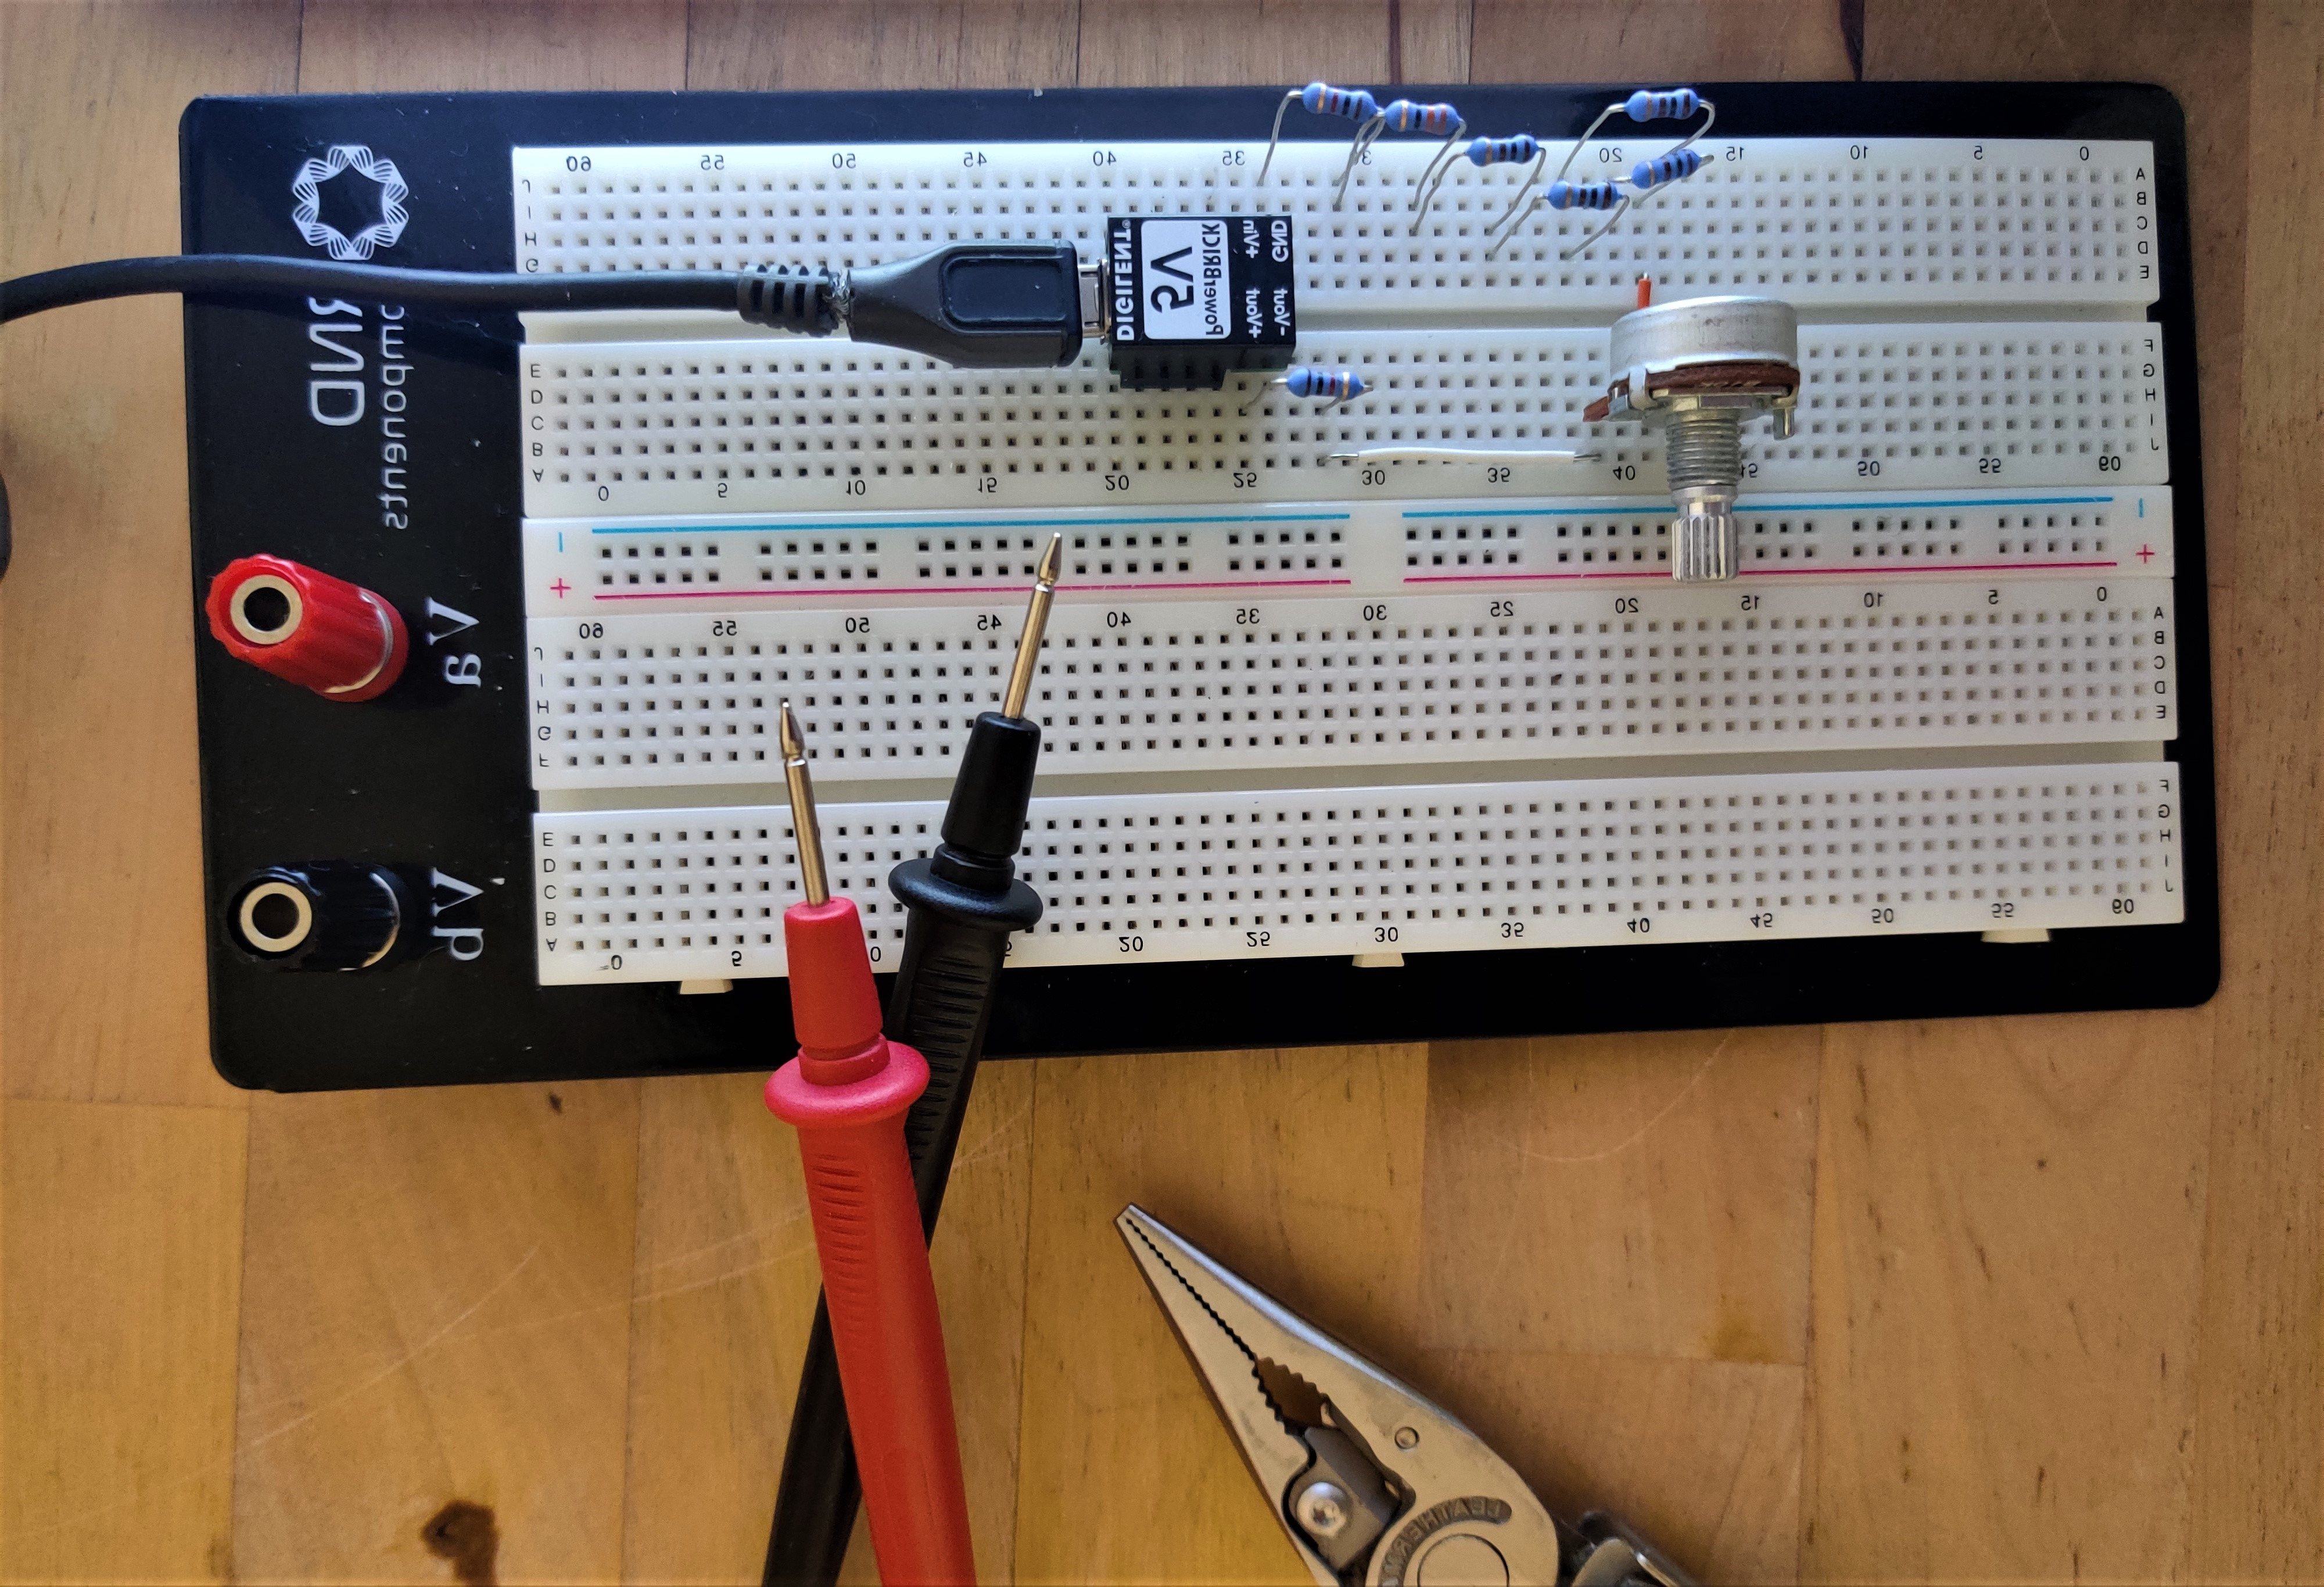
\includegraphics[scale=0.085]{D1/Images/oppkobling.jpg}
  \caption{Oppkobling av realisert krets på brødbrett.}
  \label{fig:oppkobling}
\end{figure}

\begin{table}[H]
  \centering
  \caption{Komponenter og deres standardverdier, samt målte verdier.}
  \label{tab:komp}
  \begin{tabular}{|c|c|c|}
    \hline\hline
    \textbf{Komponenter} & \textbf{Standardverdi} & \textbf{Målt verdi} \\
    \hline\hline
    $R1$   & $1M$ $\Omega$ & $930M$ $\Omega$\\
    \hline
    $R2$   & $0-10k$ $\Omega$ & $0-10.27$ $\Omega$\\
    \hline
    $R3$   & $0-10k$ $\Omega$ & $0-10.02$ $\Omega$\\
    \hline
    $L$   & $100$ mH       & $206$ mH\\
    \hline
    $C1$   & $33$ nF       & $25.48$ nF\\
    \hline
    $C2$   & $47$ nF       & $48.39$ nF\\
    \hline
    $C3$   & $5$ nF       & $4.92$ nF\\
    \hline\hline
    \textbf{Komponent} & \textbf{Navn produsent} &\\
    \hline
    CD4011UBE & Texas Instruments &\\
    \hline\hline
  \end{tabular}
\end{table}
\subsection{Test}
\label{test}

For å teste hvordan systemet fungerer undersøkes det først hvordan hvert delsystem fungerer, deretter hvordan de fungerer sammen. 

det første delsystemet som undersøkes er firkantgeneratoren. Med likning (\ref{eq:T_firkant}) kan periodetiden $T$ til firkantgeneratoren regnes ut. Dermed gir lave verdier på $R_1$ og $C_1$ i firkantgeneratoren kortere periodetid. En lav kondensatorverdi og motstandsverdi vil også være hensiktsmessig for å få skarpere kanter i firkantsignalet da den vil lade seg opp og ut raskere. 

I realisering ble en kondensatorverdi $C_1 = 25.48$nF og motstandsverdien $R_1$ satt til $930$M$\Omega$ som gir en periodetid på
\begin{equation}
    T = 2\text{ln}(3)\cdot31.48\text{nF}\cdot331.2\text{k}\Omega \approx 52ms.
\end{equation}
Fra osciloskopsanalyse til realisert firkantsignal $z(t)$ i figur \ref{fig:firkantsignal} virker det som likning (\ref{eq:T_firkant}) stemmer godt. 
\begin{figure}[H]
  \centering 
  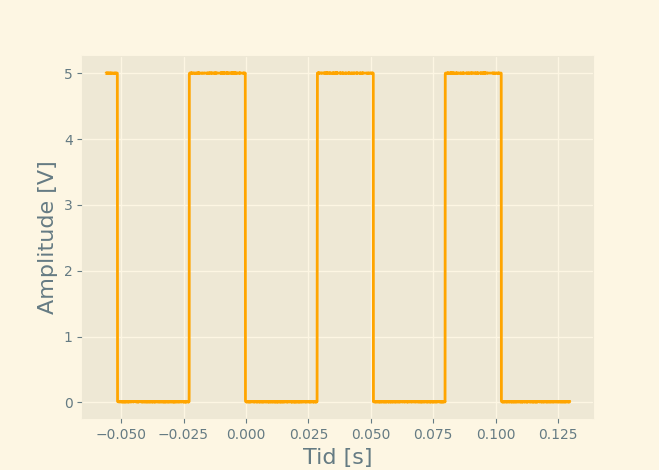
\includegraphics[scale=0.65]{D1/firkantsignal.png}
  \caption{Oscilloskopsanalyse av utgangssignalet til firkantgeneratoren $z(t)$.}
  \label{fig:firkantsignal}
\end{figure}
Impulsgeneratoren tar inn $z(t)$ som vist i figur \ref{fig:impulsgenerator}. I realiseringen ble kondensatoren $C_2 = 48.39$nF og resistoren satt til $R_2 = 10.10\text{k}\Omega$ som ga signalet vist i figur \ref{fig:s(t)}.
\begin{figure}[H]
  \centering
  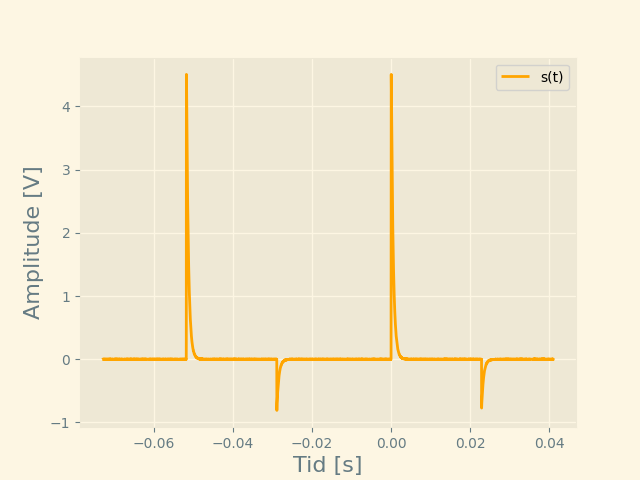
\includegraphics[scale=0.65]{D1/Images/s(t).png}
  \caption{Osciloskopsanalyse av s(t) i impulsgeneratoren.}
  \label{fig:s(t)}
\end{figure}
Figur \ref{fig:s(t)} gir en positiv amplitude når signalet skrur seg på, men også en mindre negativ amplitude når signalet går av igjen. 
Impulsgeneratoren gir ut signalet $x(t)$ vist i figur \ref{fig:x(t)} over amplitudespekteret til henholdsvis $x(t)$ under. En ideel dirac-puls ville da gitt et mer flatt amplitudespekter, men teorien om at impulser lager et flatt spekter stemmer.
\begin{figure}[H]
  \centering
  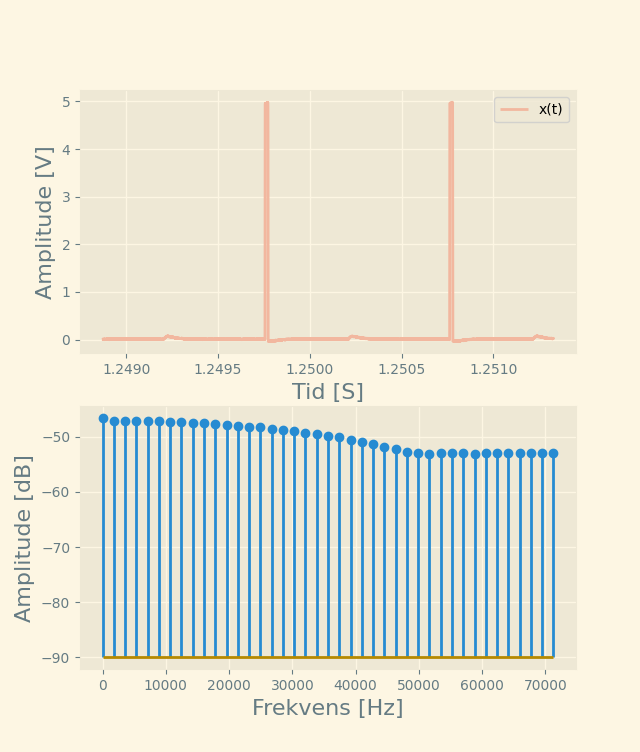
\includegraphics[scale=0.65]{D1/Images/x(t).png}
  \caption{Osciloskopsanalyse av utgangen $x(t)$ til impulsgeneratoren med amplitudespekteret til $x(t)$ under.}
  \label{fig:x(t)}
\end{figure}
Impulsene som ble generert, vist i figur \ref{fig:impulsrespons}, kan leses av fra oscilloskopet til å ha en varighet på omtrent $340\mu$s og med $\tau = 4.887^{-4}$s kan likning (\ref{eq:finishedTau}) gi:
\begin{equation}
    \text{ln}(2)4.887^{-4}s\approx340\mu\text{s}.
\end{equation}
\begin{equation}
    338\mu s \approx 340\mu s.
\end{equation}
Med andre ord stemmer teorien med praksis i dette tilfelle godt, da avviket kan være målefeil fra oscilloskopet eller komponentverdiene.

Impulsene fra $x(t)$ blir sendt gjennom RLC-filteret som gir impulsresponsene vist i figur \ref{fig:impulsrespons} med forskjellige verdier for $R_3$. Ved å endre på $R_3$ endres Q-verdien til filteret som fører til at svingningene dempes raskere. Kondensatoren $C_3$ og spolen $L$ er valgt fra gitt senterfrekvens på $5050$Hz som blir nøyere beskrevet i~\cite{D2}.
\begin{figure}[H]
  \centering
  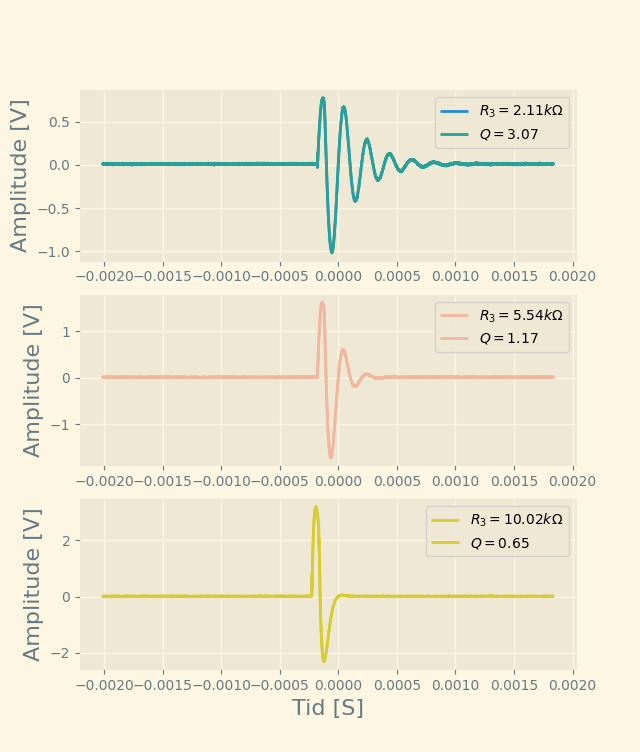
\includegraphics[scale=0.65]{D1/Images/Dempningsfaktor.png}
  \caption{Osciloskopsanalyse av s(t) i impulsgeneratoren med resistorverdi og Q-verdi.}
  \label{fig:impulsrespons}
\end{figure}

\section{Konklusjon}
\label{sec:konklusjon}
Ideen om å bruke CD4011UBE samt motstander og resistorer for å finne impulsresponsen til et andreordens RLC-båndpassfilter med gitt senterfrekvens stemte. Det er derimot viktig å velge riktige kondensator- og motstandsverdier for at kretsen skal kunne generere impulser. Hvor godt det fungerte vil variere fra hva det skal brukes til, men det fungerer til å finne impulsresponsen til et RLC-filter. 

Periodetiden $T$ til firkantsignalet må være langt nok til at det ikke interferer med lengden på impulsresponsen. 
Hvor korte impulser som er mulig å få til i praksis er vanskelig å vite, men det er mulig å få til veldig korte impulser ved å gjøre $\tau$ så lav som mulig i høypassfilteret til impulsgeneratoren. 
Det er også mulig å finne et matematisk utrykk for pulsbredden som funksjon av tidskonstanten $\tau$ vist i likning (\ref{eq:finishedTau}). Realisert pulsbredde ble $340\mu$s som var tilstrekkelig kort for å kunne se på impulsresponsen til et RLC-filter.
Spektrumet til impulsene var tilnærmet flatt, som vist i figur \ref{fig:impulsrespons}, men ikke så flatt som en ideel dirac-puls ville hatt.  

\phantomsection
\addcontentsline{toc}{section}{Referanser}

\begin{thebibliography}{99}
    \bibitem{Ert-18}
        \textit{ERT-økt 18: En klokkegenerator}, 
    	NTNU,
    	2022.
    \bibitem{Ert-19}
        \textit{ERT-økt 19: Transienter i første ordens system}, 
    	NTNU,
    	2022.
    \bibitem{Eksamensprosjekt}
        \textit{Eksamensprosjekt}, 
    	TTT4260, NTNU,
    	2022.
    \bibitem{datablad}
        Texas Instruments, 
        \textit{CMOS Quad 2-input NAND Gate}, 
    	2003.
    \bibitem{D2}
        Fløan F., 
        \textit{Designprosjekt 2: Støyfjerningsfilter}, 
    	NTNU,
    	2022.
    \bibitem{D3}
        Fløan F., 
        \textit{Designprosjekt 3: Frekvensmultiplikator}, 
    	NTNU,
    	2022.
    \bibitem{oving6}
        \textit{Øving 6}, 
    	TTT4265 – Elektronisk systemdesign og -analyse I,
    	2022.
    \bibitem{D4}
        Fløan F., 
        \textit{Designprosjekt 4: Piparen}, 
    	NTNU,
    	2022.
\end{thebibliography}

\end{document}